\Chapter{Proposed Method}\label{chapter:proposed-method}

In this chapter, I describe the proposed method for adapting a pre-trained 2D diffusion model to understand 3D geometry and synthesize novel views of objects. The approach focuses on conditioning the generative process on both a reference image and relative camera transformations.

\section{Overview}
The core challenge in adapting 2D diffusion models for novel view synthesis lies in equipping them with an understanding of 3D space and object geometry.
This work proposes a method that augments a pre-trained text-to-image diffusion model, specifically Stable Diffusion 2.1, with two primary conditioning mechanisms: one for visual appearance derived from a source reference image, and another for geometric understanding derived from camera pose information.
By integrating these conditioning signals, the model learns to generate novel views of an object from a given source image and a target camera pose.
The overall architecture is designed to be efficient by primarily training lightweight adapter modules and specialized encoders, while keeping the majority of the large pre-trained model frozen to preserve its generative priors and ensure computational efficiency during training.

\section{Limitations of Previous Methods}\label{sec:limitations}

Despite the significant progress in multi-view image generation and novel view synthesis, several limitations and research gaps remain:

\begin{enumerate}
  \item \textbf{Computational Efficiency}: Full fine-tuning of diffusion models for multi-view generation is computationally expensive, especially when working with large base models and high-resolution images. While first adapter-based method MV-Adapter has improved efficiency of training, there is still room for improvement.

  \item \textbf{Geometric Consistency}: Maintaining geometric consistency across generated views remains a challenge, particularly when generating views from significantly different perspectives. Current methods often struggle with complex occlusions, reflective surfaces and fine geometric details.

  \item \textbf{Lighting issues}: The lighting plays a critical role in the visual appearance of rendered objects. The example rendering scripts provided by the ObjaverseXL authors \cite{objaverse} employed a randomized lighting setup. While intended to introduce variability, this approach often resulted in images with harsh lighting, strong shadows, or scenes where the object was underexposed or even completely obscured because the light source was positioned unfavorably. This can negatively impact the 3D reconstruction from images since the Novel View Synthesis should provide meaningful information about texture and geometry.

  \item \textbf{Adaptation to unseen objects}: The current methods are not able to generalize to unseen objects, which is a major limitation.

  \item \textbf{Adaptation to different viewpoints}: The current methods are not able to adapt to different viewpoints, which is a major limitation. If a given method was trained on specific set of perspectives it cannot generalize to the new viewpoints.
\end{enumerate}

My work aims to adress the \textbf{Computational Efficiency} by using only trainable adapter layers, \textbf{Lighting issues} by ensuring consistent lighting in datasets, and \textbf{Adaptation to different viewpoints} by conditioning the model on many camera parameter configurations.
The problem of \textbf{Adaptation to unseen objects} can be adressed by large-scale training on a diverse set of objects.

\section{Architectural Framework}\label{sec:architectural-framework}
The proposed method leverages the strong generative capabilities of a pre-trained 2D diffusion model and extends it for 3D-aware novel view synthesis. This is achieved through the introduction of specialized conditioning modules that inject visual and geometric information into the denoising U-Net.

\subsection{Introduction and System Diagram}
The primary goal is to adapt the Stable Diffusion 2.1 model, an inherently 2D generative framework, to comprehend 3D spatial relationships and generate images from novel viewpoints. The system achieves this by integrating two distinct conditioning streams into the diffusion model's U-Net architecture. The first stream provides visual context from a source (reference) image, while the second stream imparts geometric awareness through encoded camera parameters.
Figure \ref{fig:my-method-diagram} illustrates the overall architecture of the proposed system, highlighting the flow of information and the interplay between the original diffusion model components and the newly introduced conditioning modules.

\begin{figure}[htbp]
  \centering
  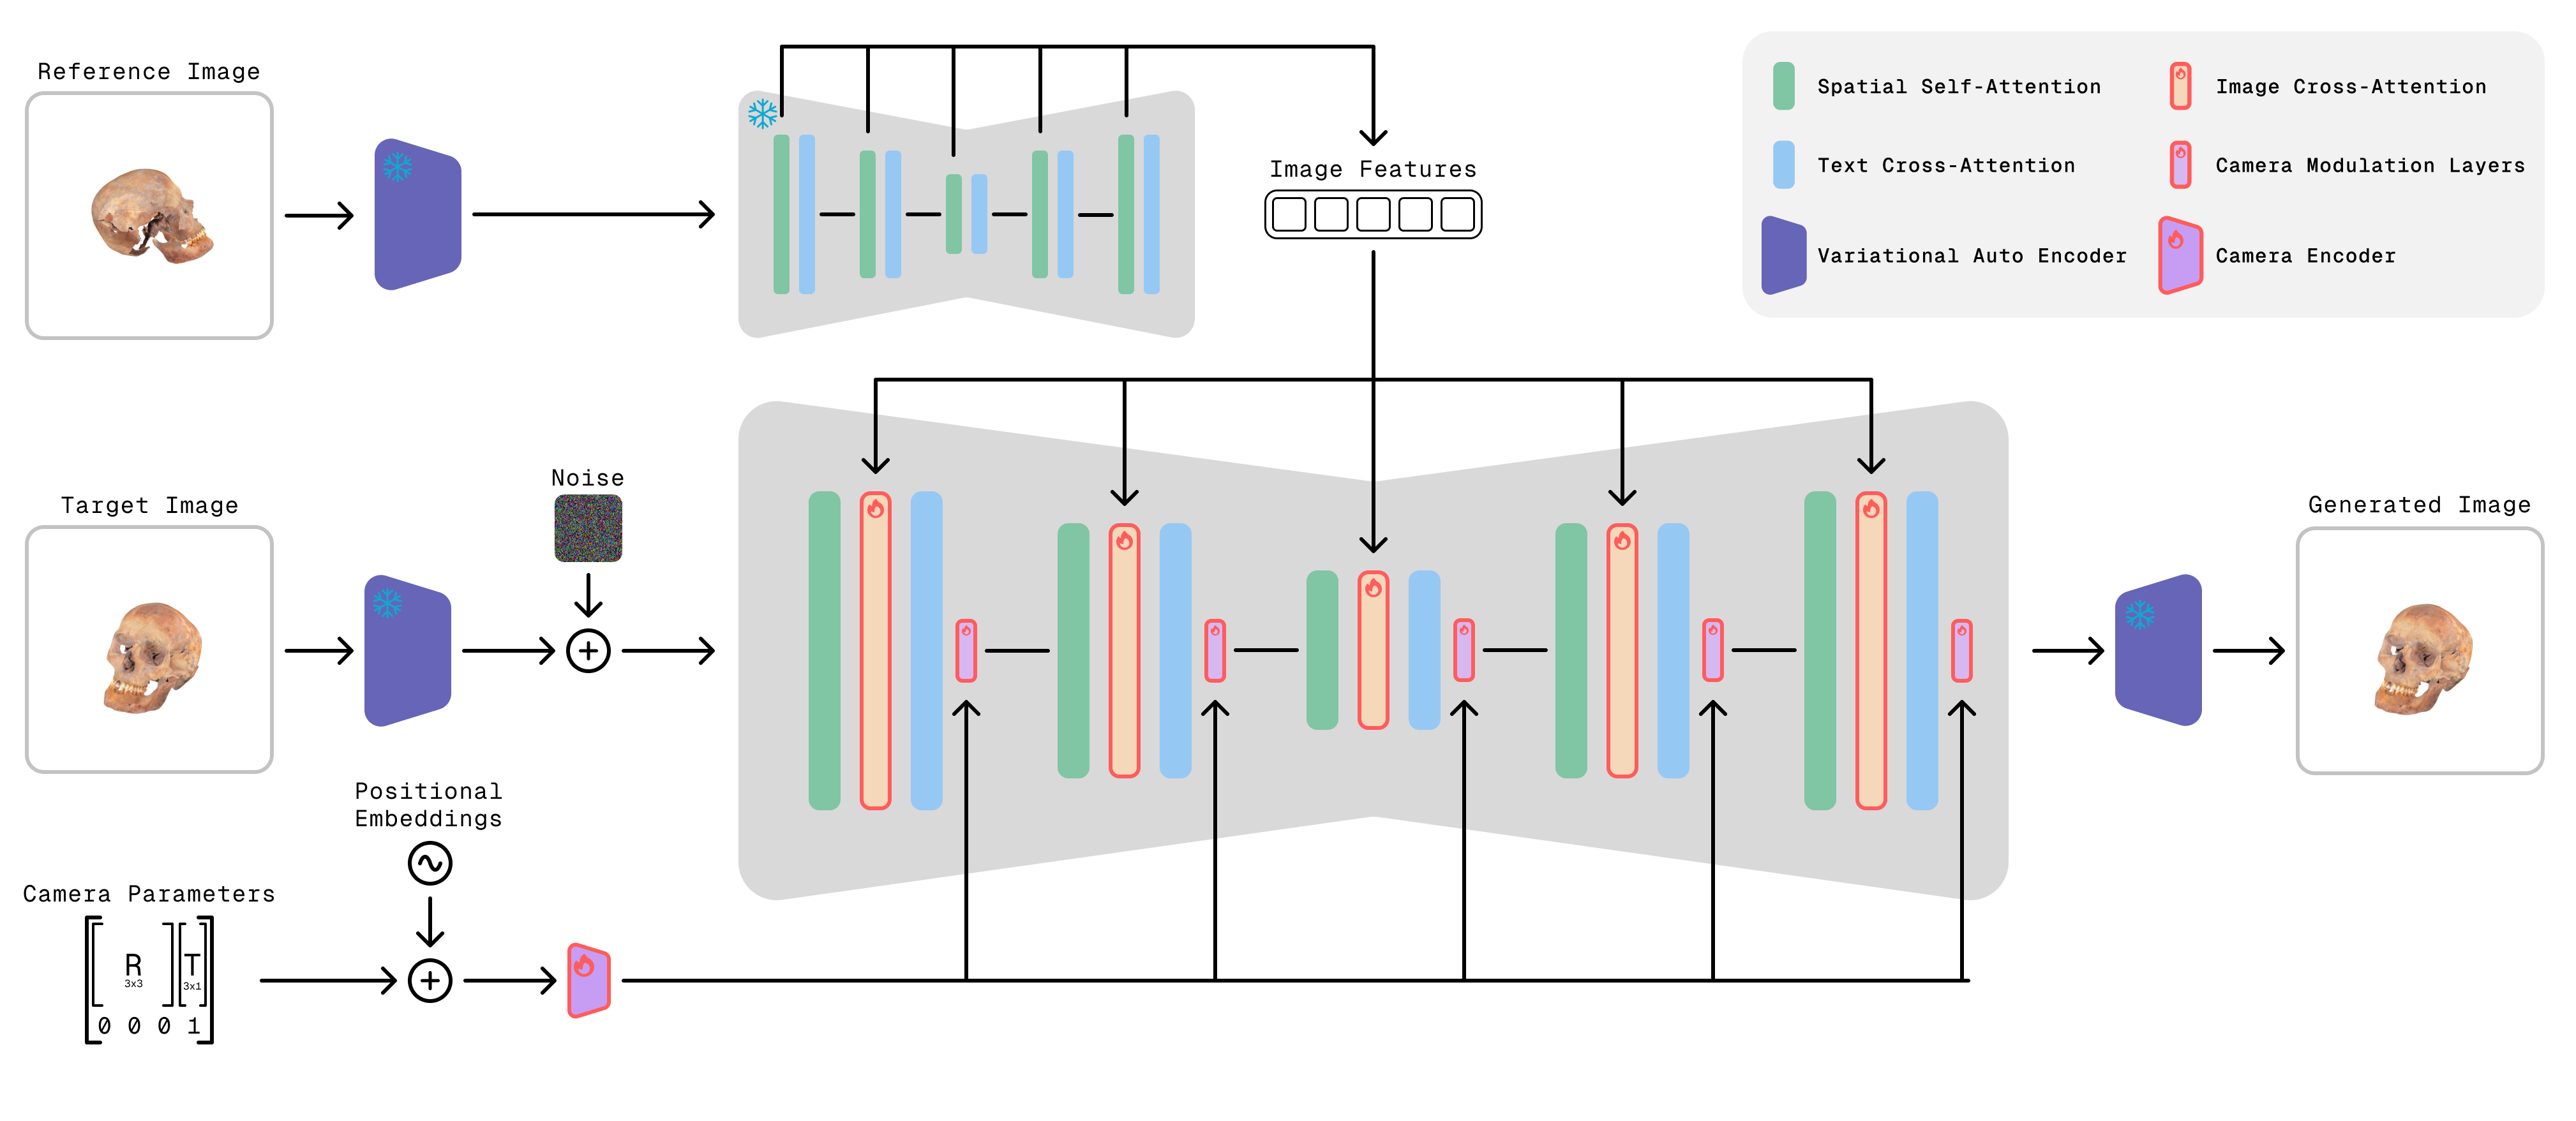
\includegraphics[width=\textwidth]{images/proposed-method/my-method-diagram.png}
  \caption{System diagram of the proposed multi-view diffusion model. It showcases the reference image encoding path, the camera parameter encoding path, and their integration into the main denoising U-Net.}
  \label{fig:my-method-diagram}
\end{figure}

\subsection{Backbone: Stable Diffusion 2.1}
The foundation of proposed method is the Stable Diffusion 2.1 model. This choice is motivated by its robust text-to-image generation capabilities and its publicly available pre-trained weights, which encapsulate a vast understanding of visual concepts. The core component relevant to my modifications is its U-Net architecture \cite{unet}, which performs the iterative denoising process.
In my approach, several key components of the original Stable Diffusion 2.1 model are kept frozen to preserve their learned knowledge and ensure computational efficiency during training. These include the Variational Autoencoder (VAE) \cite{vae} used for encoding images into and decoding latents from the latent space, the text encoder CLIP \cite{clip} responsible for processing textual prompts, and the weights of the original U-Net when used within the Reference Image Encoder. The new conditioning modules and adapters are specifically designed to be trainable.

\subsection{Reference Image Conditioning Stream}
To enable the model to generate views that are visually consistent with a given input, a reference image conditioning stream is introduced. This stream aims to capture and transfer the appearance, texture, color, and identity of the object depicted in the source image to the novel view generation process.

\subsubsection{Source Image Feature Extraction}
The process of extracting visual features from the source image is handled by a dedicated $ImageEncoder$ module. This module operates as follows:
\begin{enumerate}
  \item The source image is first transformed into a latent representation using the frozen VAE of the backbone Stable Diffusion model. This compresses the image into a lower-dimensional space where the diffusion process typically operates.
  \item This latent representation is then processed by the original, frozen U-Net of Stable Diffusion 2.1. Critically, this forward pass through the U-Net is performed with the timestep parameter set to zero ($t=0$). This effectively instructs the U-Net to perform a "denoising" pass on the clean latent, attending to the image and extracting rich, multi-scale visual features.
  \item During this pass, the $ImageEncoder$ captures the output activations from the self-attention layers present within each block of the frozen U-Net. These extracted features, which encode comprehensive visual information about the source image at different semantic levels, are then made available for conditioning the main denoising process.
\end{enumerate}

\subsubsection{Image Cross-Attention Adapters}
The visual features extracted by the $ImageEncoder$ are injected into the main denoising U-Net using newly introduced, trainable adapter modules that serve as cross-attention layers. These processors are designed to be lightweight and are integrated into each corresponding block of the denoising U-Net.
A key architectural choice is the parallel integration of these image cross-attention adapters. Instead of serially passing information through the original attention layers and then the new adapters, the adapters operate in parallel to the U-Net's existing self-attention and text-cross-attention mechanisms. The extracted image features serve as the key and value for these new cross-attention layers, while the U-Net's intermediate hidden states act as the query. This allows the denoising U-Net to directly attend to relevant visual details from the source image at multiple stages of the generation process, with the influence of these reference features controlled by a scaling factor, which was tested in the range of $0.1$ to $1.0$ during training.

\subsection{Camera Parameter Conditioning Stream}
To ensure geometric consistency and enable precise control over the viewpoint of the generated image, a camera parameter conditioning stream is employed. This stream encodes the relative transformation between the source and target camera poses and uses this information to modulate the behavior of the denoising U-Net.

\subsubsection{Camera Pose Encoding}
The $CameraEncoder$ module is responsible for processing the geometric information.
The input to this module is the relative camera transformation from the source view to the target view, represented by a $3 \times 3$ rotation matrix $R$ and a $3 \times 1$ translation vector $T$. These $12$ parameters ($9$ for $R$ and $3$ for $T$) define the desired viewpoint change.
To enrich this relatively low-dimensional signal, rotary positional embeddings are applied to the camera parameters. This augmentation aims to provide a more distinctive and structured representation for the subsequent neural network layers.
The enriched camera parameters are then processed by a Multi-Layer Perceptron (MLP). This MLP typically consists of several layers with SiLU activation functions, transforming the camera pose information into a high-dimensional embedding suitable for conditioning.

\subsubsection{FiLM-based Network Modulation}
The high-dimensional camera embedding produced by the $CameraEncoder$ is used to modulate the activations within the main denoising U-Net via Feature-wise Linear Modulation (FiLM) layers \cite{film}. For a given feature map $h$ in the U-Net, the FiLM layer applies an affine transformation:
\[ FiLM(h) = \gamma \cdot h + \beta \]
where $\gamma$ (scale) and $\beta$ (shift) are parameters generated by passing the camera embedding through dedicated linear layers within the $CameraEncoder$.
These FiLM modulations are applied at each UNET block to the outputs of the feature maps (down-sampling, middle, and up-sampling blocks).

This allows the camera pose information to dynamically influence the feature representations throughout the network, guiding the geometric aspects of the image generation. The strength of this modulation can be adjusted by a scalar factor, which was tested in the range of $0.1$ to $1.0$ during training.

\subsection{The Integrated Conditioned U-Net}
The $MultiViewUNet$ module serves as the central component of the proposed architecture. It integrates the backbone Stable Diffusion U-Net with the two conditioning streams described above: the reference image conditioning via parallelly connected Image Cross-Attention Adapters and the camera parameter conditioning via Feature-wise Linear Modulation (FiLM) layers.

During each step of the reverse diffusion process, the $MultiViewUNet$ takes the noisy latent representation of the target image, the current timestep, text embeddings, the extracted reference image features, and the encoded target camera parameters. It then predicts the noise present in the noisy latent. The system diagram in Figure \ref{fig:my-method-diagram} provides a visual summary of this integrated data flow.

\section{Model Training}
The training process is designed to teach the $MultiViewUNet$ to effectively utilize the visual and geometric conditioning information to predict the noise required to generate a target view from a source view and camera transformation.

\subsection{Training Objective and Loss Functions}
The primary training objective is to minimize the difference between the noise predicted by the $MultiViewUNet$ and the actual noise that was added to the target image's latent representation. This is typically formulated as a Mean Squared Error (MSE) loss:
\[ L_{noise} = \mathbb{E}_{x_0, \epsilon, t} [\| \epsilon - \epsilon_\theta(x_t, t, c_{img}, c_{cam}, c_{text}) \|^2] \]
where $x_0$ is the clean target image latent, $\epsilon$ is the sampled Gaussian noise, $t$ is the timestep, $x_t$ is the noisy latent at timestep $t$, and $\epsilon_\theta$ is the noise predicted by the network conditioned on image features $c_{img}$, camera embedding $c_{cam}$, and text embedding $c_{text}$.
The noise scheduler is configured to predict the noise term $\epsilon$.

To improve training stability and sample quality, especially at varying noise levels, an SNR-aware weighting strategy is employed for the loss function, specifically the Min-SNR-$\gamma$ approach \cite{minsnr}. The loss for each training instance is weighted by $min(SNR_t, \gamma) / SNR_t$, where $SNR_t$ is the signal-to-noise ratio at timestep $t$, and $\gamma$ is a hyperparameter (e.g., set to $5.0$) as the method authors recommend \cite{minsnr}. This weighting scheme effectively gives more importance to timesteps with lower SNR values, preventing the model from focusing excessively on high-SNR (low noise) timesteps. The noise schedule itself is a DDPMScheduler, further modified using an interpolated shift based on the SNR, with a shift scale factor (e.g., $6.0$), which adapts the noise levels experienced during training.

While the primary loss focuses on noise prediction, auxiliary metrics such as  Peak Signal-to-Noise Ratio (PSNR), perceptual loss (LPIPS \cite{lpips}), Structural Similarity Index Measure (SSIM \cite{ssim}), CLIP score \cite{clipscore}, and Frechet Inception Distance (FID \cite{fid1, fid2}) are monitored upon validation steps to provide a more comprehensive assessment of image quality and consistency.

\subsection{Training Data and Iteration}
Each training iteration involves a batch of data samples. A single sample consists of:
\begin{itemize}
  \item A source image.
  \item A target image (representing a different view of the same object).
  \item The relative camera transformation (rotation $R$ and translation $T$) from the source camera pose to the target camera pose.
  \item A textual prompt describing the object (leveraging the underlying text-to-image capabilities of Stable Diffusion).
\end{itemize}
The model is trained to predict the noise in the target image's latent, conditioned on the source image, the camera transformation, and the text prompt.

\subsection{Optimization and Implementation Details}
The trainable parameters of the model include the weights of the modules mentioned in Section \ref{sec:architectural-framework}. The core U-Net of Stable Diffusion 2.1, the VAE, and the text encoder remain frozen during this fine-tuning phase.
Optimization is performed using the AdamW optimizer \cite{adamw} with a learning rate of $1 \times 10^{-5}$. A cosine learning rate schedule with a warm-up period is employed to manage the learning rate dynamics over the training duration, which is set for a total of $10$ epochs. Gradient clipping is applied with a maximum norm of $1.0$ to prevent exploding gradients. Training is performed using a batch size of $6$ per GPU. Model was trained on 4 GPUs (NVIDIA A100 40GB). The model is implemented using PyTorch and PyTorch Lightning, and leverages mixed-precision training (e.g., $float32$) for efficiency.

\section{Inference Process}
Once trained, the model can be used to synthesize a novel view of an object from a given source image and a specified target camera pose.

\subsection{Novel View Synthesis Pipeline}
The inference process, managed by the $MVDPipeline$, proceeds as follows:
\begin{enumerate}
  \item \textbf{Inputs}: The pipeline takes a single source image, the desired target camera parameters, and an optional text prompt.
  \item \textbf{Source Image Encoding}: The source image is processed by the $ImageEncoder$ to extract its multi-scale visual features.
  \item \textbf{Camera Parameter Encoding}: The target camera transformation is encoded by the $CameraEncoder$ to produce a camera embedding.
  \item \textbf{Iterative Denoising}: Starting from a randomly sampled Gaussian noise tensor in the latent space (of the same dimensions as the VAE's output latents), the $MultiViewUNet$ iteratively denoises this latent over a predefined number of steps (in my case, $20$). In each step, the U-Net receives the current noisy latent, the timestep $t$, the text prompt embedding, the extracted source image features, and the target camera embedding (via FiLM layers). Classifier-Free Guidance (CFG) is typically used, where the model makes both a conditional and an unconditional prediction, and the final noise estimate is a weighted combination, controlled by a guidance scale (e.g., $1.0$).
  \item \textbf{VAE Decoding}: After the final denoising step, the resulting clean latent representation is decoded back into pixel space using the frozen VAE's decoder.
\end{enumerate}

\subsection{Output}
The final output of the pipeline is the synthesized image, which represents the object from the specified target viewpoint, conditioned by the appearance of the source image and guided by the geometric transformation.
The output images are generated at a resolution consistent with the training data, maximum supported by the model is $768 \times 768$ pixels.
